\documentclass{beamer}
\title{Urbanization from the Bottom Up}
\author{John S. Schuler \\ Department of Computational and Data Sciences \\ George Mason University}
\date{\today}

\usepackage{tikz}
\usetikzlibrary{arrows.meta, positioning, shapes.geometric, fit, backgrounds, matrix}
\usepackage{pgfplots}
\pgfplotsset{compat=1.10}
\usepackage{booktabs}
\usepackage{xcolor}
\usepackage{amsmath}
\usepackage{amssymb}
\usepackage{latexsym}
\usepackage{graphicx}

\DeclareMathOperator*{\argmax}{arg\,max}
\DeclareMathOperator*{\argmin}{arg\,min}

\setbeamercolor{background canvas}{bg=black}
\setbeamercolor{normal text}{fg=white}
\setbeamercolor{title}{fg=gray}
\setbeamercolor{frametitle}{fg=gray}
\setbeamercolor{subtitle}{fg=gray}
\setbeamercolor{item}{fg=white}
\setbeamercolor{subitem}{fg=white}

% convenience colors
\definecolor{nimbyblue}{RGB}{100,180,255}
\definecolor{nimbygray}{RGB}{180,180,180}
\definecolor{nimbygreen}{RGB}{100,220,150}
\definecolor{nimbyred}{RGB}{255,100,100}
\definecolor{nimbyyellow}{RGB}{255,220,80}

\begin{document}

% -----------------------------------------------------------------------
\begin{frame}
  \titlepage
\end{frame}

% =====================================================================
%  SECTION 1 — EMPIRICAL MOTIVATION
% =====================================================================

\begin{frame}
  \frametitle{Outline}
  \begin{enumerate}
    \item Empirical motivation: what happened to housing?
    \item The NIMBY ABM: model design and mechanics
    \item Building with generative AI
    \item Parameter sweeps: what we learn overnight
    \item Connections and future work
  \end{enumerate}
\end{frame}

% --- slide: Fairfax County prices ------------------------------------
\begin{frame}
  \frametitle{Fairfax County Home Prices}
  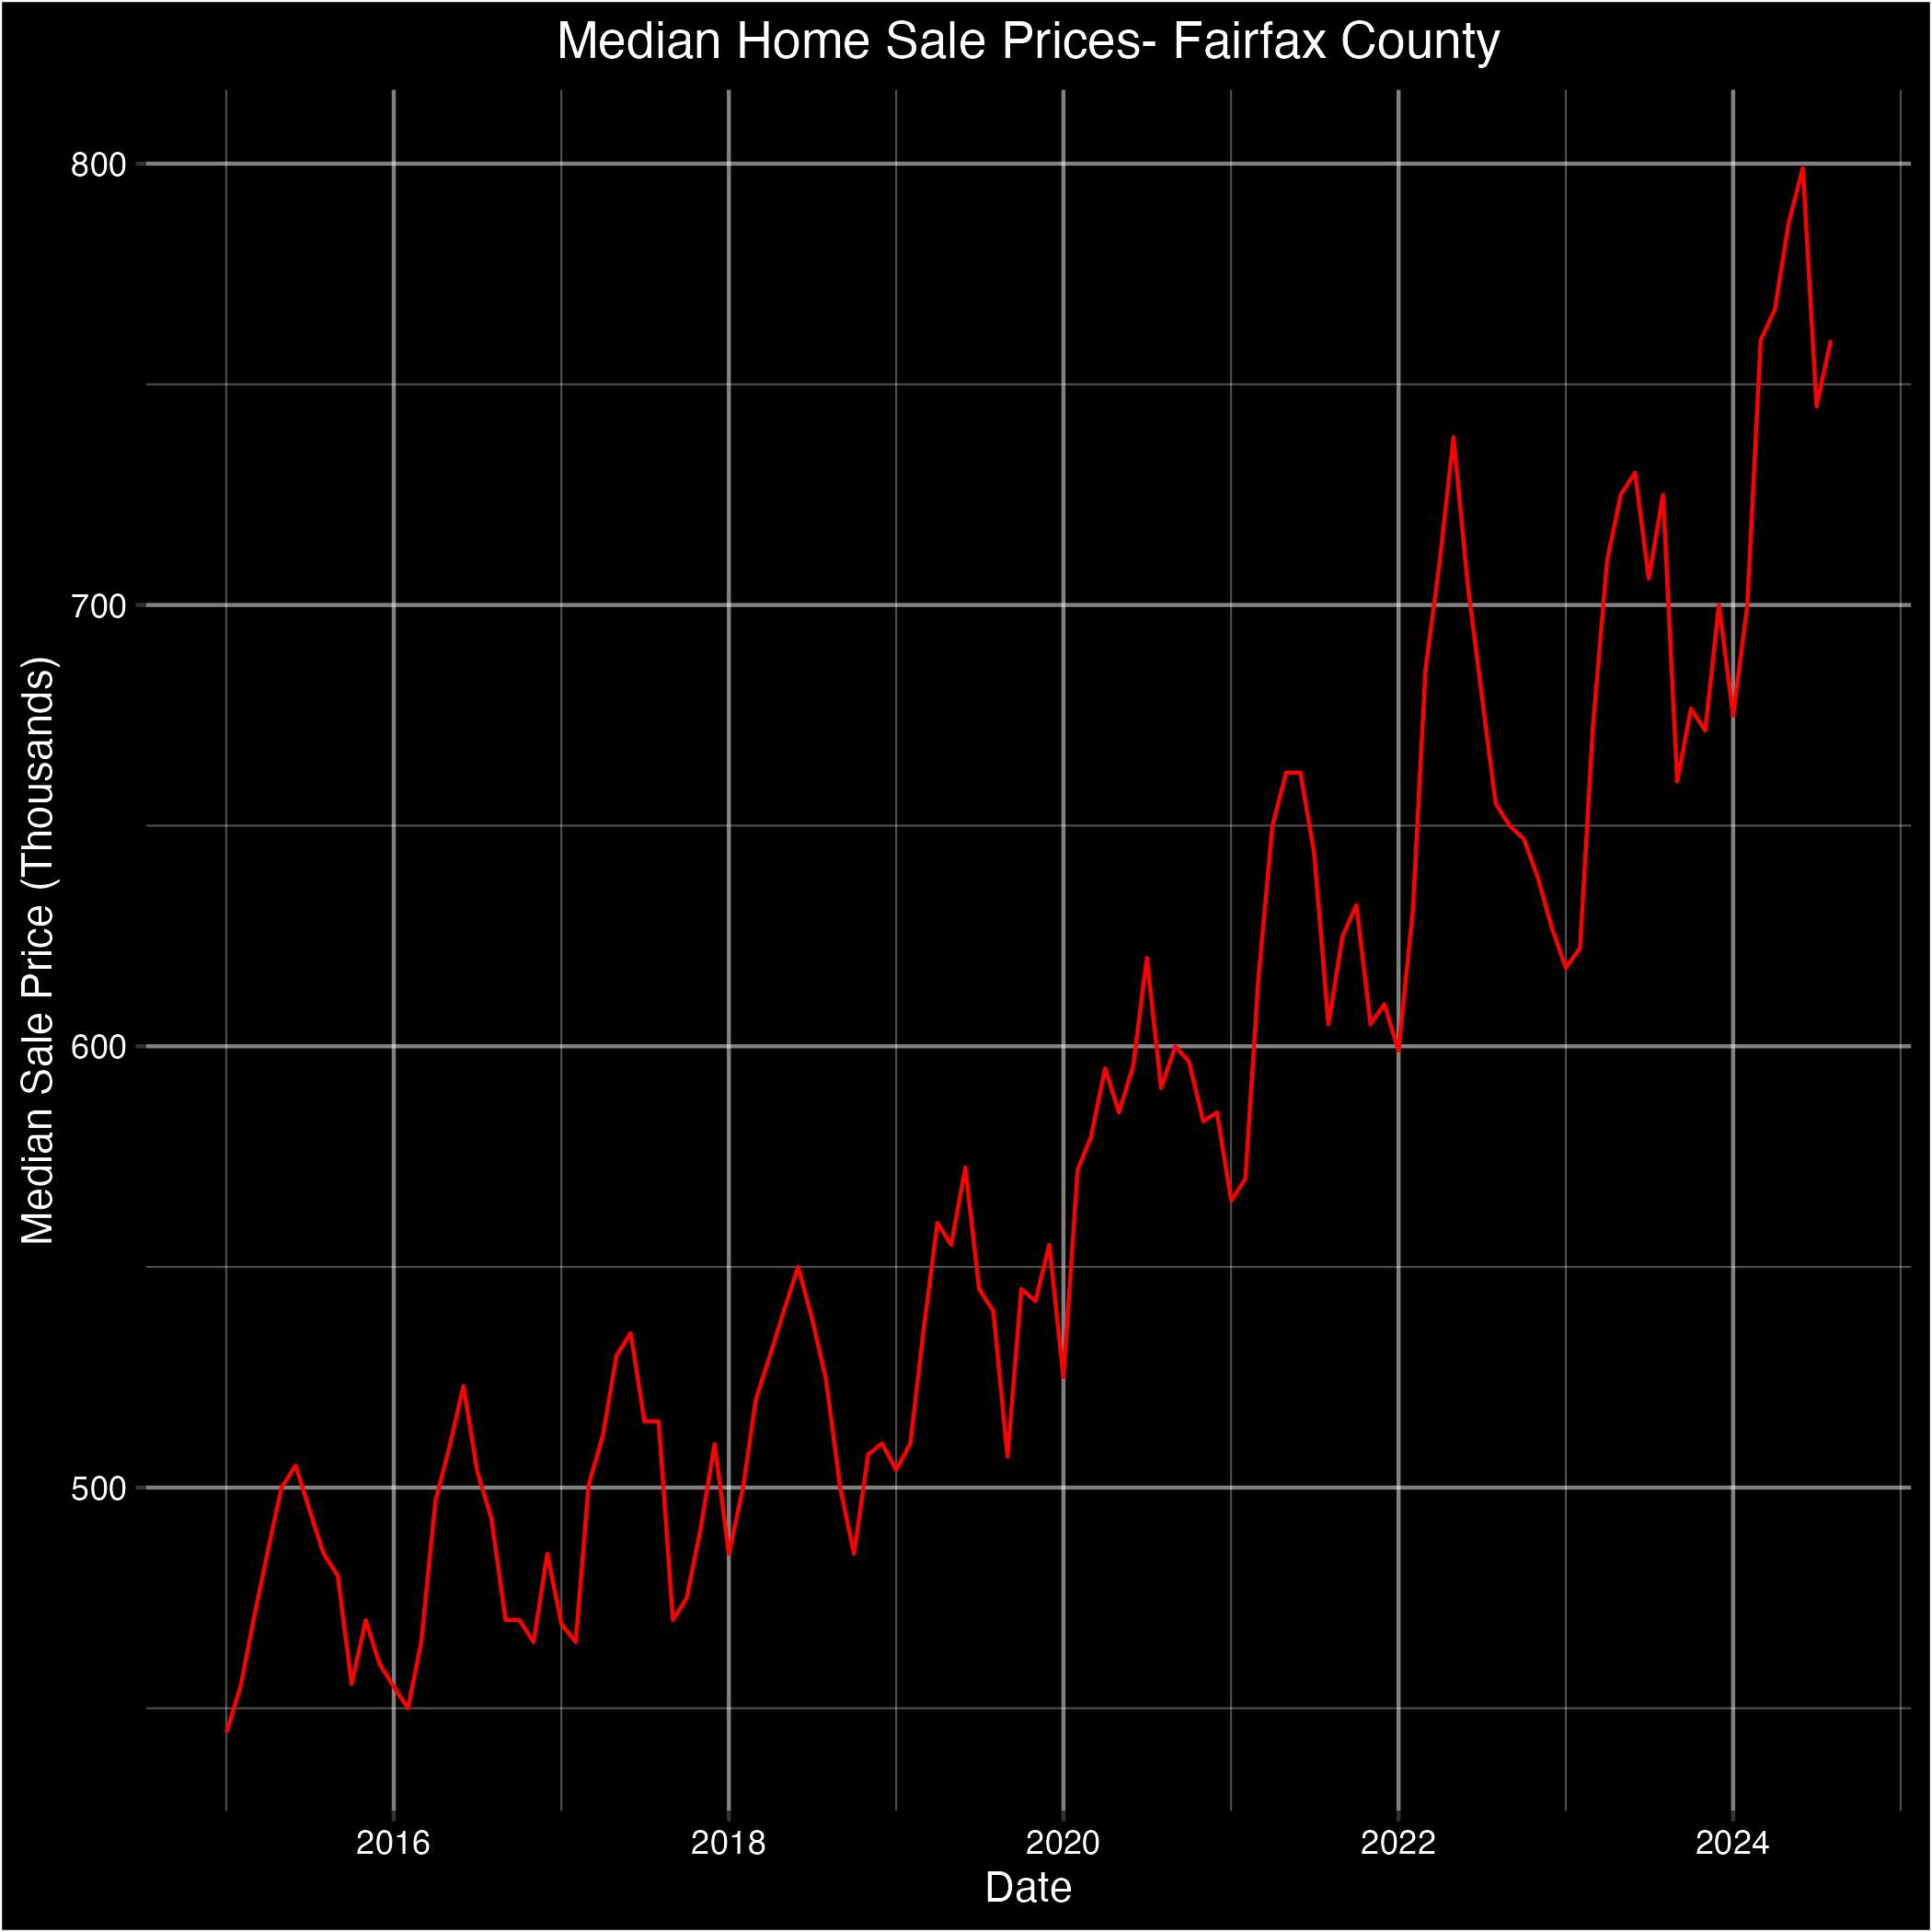
\includegraphics[width=0.90\textwidth, height=0.72\textheight, keepaspectratio]{homePrices.png}
\end{frame}


% =====================================================================
%  SECTION 2 — THE MODEL
% =====================================================================

\begin{frame}
  \frametitle{Why Agent-Based Modeling?}
  \begin{columns}
    \column{0.5\textwidth}
    \textcolor{nimbygray}{Standard models assume:}
    \begin{itemize}
      \item Homogeneous agents
      \item Perfect information
      \item Instantaneous market clearing
      \item Zoning as an exogenous constraint
    \end{itemize}
    \column{0.5\textwidth}
    \textcolor{nimbygreen}{Housing is fundamentally:}
    \begin{itemize}
      \item Heterogeneous (location, type, vintage)
      \item Locally governed (neighborhood politics)
      \item Path-dependent (who is already there)
      \item Endogenous supply (residents vote on zoning)
    \end{itemize}
  \end{columns}
  \vspace{0.6em}
  \begin{center}
    \textcolor{nimbyyellow}{ABM lets residents, buildings, and laws co-evolve.}
  \end{center}
\end{frame}

% --- slide: city structure -------------------------------------------
\begin{frame}
  \frametitle{City Structure}
  \begin{center}
  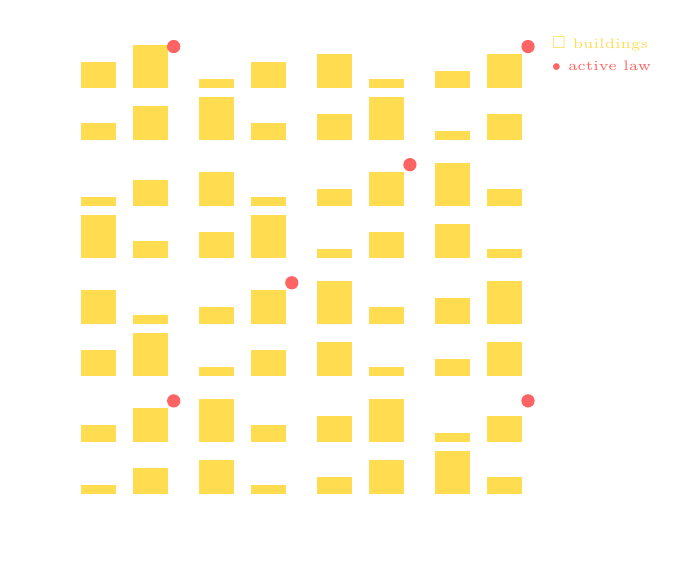
\begin{tikzpicture}[scale=0.60]
    % 4x4 neighborhoods, each with 2x2 buildings — tighter spacing, yellow buildings
    \foreach \nx in {0,1,2,3} {
      \foreach \ny in {0,1,2,3} {
        % neighborhood border
        \draw[white, thick] (\nx*2.5, \ny*2.5)
          rectangle (\nx*2.5+2.4, \ny*2.5+2.4);
        % 2x2 buildings inside
        \foreach \bx in {0,1} {
          \foreach \by in {0,1} {
            \pgfmathsetmacro{\ht}{mod(\nx*3+\ny*7+\bx*2+\by,5)+1}
            \fill[nimbyyellow]
              (\nx*2.5+\bx*1.1+0.18, \ny*2.5+\by*1.1+0.18)
              rectangle
              (\nx*2.5+\bx*1.1+0.92, \ny*2.5+\by*1.1+0.18+\ht*0.18);
          }
        }
        % law indicator dot
        \pgfmathtruncatemacro{\haslaw}{mod(\nx+\ny*2,3)}
        \ifnum\haslaw=0
          \fill[nimbyred] (\nx*2.5+2.15, \ny*2.5+2.15) circle (4pt);
        \fi
      }
    }
    % labels
    \node[color=white, font=\small] at (4.8, -0.5) {$n \times n$ neighborhoods};
    \node[color=nimbygray, font=\tiny, align=left] at (11.2, 9.5)
      {\textcolor{nimbyyellow}{$\square$ buildings}\\[2pt]\textcolor{nimbyred}{$\bullet$ active law}};
    \draw[<->, white, thick] (-0.3,0) -- (-0.3,2.4) node[midway, left, font=\tiny, color=white] {$k$};
  \end{tikzpicture}
  \end{center}
  \vspace{-0.3em}
  \small Default: $10\times10$ neighborhoods, each $8\times8$ buildings = \textbf{6,400 buildings}.\\
  Building \emph{height} = number of stacked dwellings. Neighbors vote on zoning laws.
\end{frame}

% --- slide: agent preferences ----------------------------------------
\begin{frame}
  \frametitle{Agent Preferences}
  Each agent $i$ has a job location and residential preferences drawn from
  log-normal / truncated-normal distributions:
  \vspace{0.3em}
  \begin{center}
  \begin{tabular}{lll}
    \toprule
    \textcolor{nimbygray}{Parameter} & \textcolor{nimbygray}{Meaning} & \textcolor{nimbygray}{Distribution} \\
    \midrule
    $b_i$ & budget & log-normal \\
    $\bar{d}_i$ & preferred neighborhood density & log-normal \\
    $\bar{h}^{\max}_i,\; \bar{h}^{\min}_i$ & preferred max/min heights & log-normal \\
    $\bar{h}_i$ & preferred building height & log-normal \\
    $\sigma^{nh}_i,\; \sigma^{b}_i$ & sensitivity to deviations & log-normal \\
    $\lambda_i$ & proximity decay scale & log-normal \\
    $\theta_i$ & Frank copula dependence & log-normal \\
    \bottomrule
  \end{tabular}
  \end{center}
  \vspace{0.4em}
  \small Job buildings assigned at creation, weighted by $w(b) = \text{height}(b) + 1$.
\end{frame}

% --- slide: utility function -----------------------------------------
\begin{frame}
  \frametitle{The Utility Function}
  \textbf{Five marginal utilities} $u_k \in [0,1]$, combined via Frank copula:
  \[
    C_\theta(u_1,\ldots,u_5)
    = -\frac{1}{\theta}\ln\!\left(1 + \frac{\prod_k(e^{-\theta u_k}-1)}{(e^{-\theta}-1)^4}\right)
  \]
  \vspace{-0.5em}
  \begin{center}
  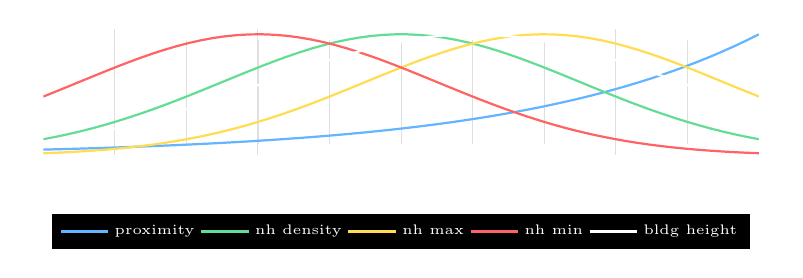
\begin{tikzpicture}
    \begin{axis}[
      width=0.88\textwidth, height=3.2cm,
      xmin=0, xmax=1, ymin=0, ymax=1.05,
      xlabel={Marginal utility $u_k$},
      ylabel={}, ytick=\empty,
      tick style={color=white}, axis line style={color=white},
      xlabel style={color=white, font=\small},
      xticklabel style={color=white, font=\small},
      grid=major, grid style={color=gray!25},
      legend style={fill=black, draw=white, text=white, font=\tiny,
                    at={(0.5,-0.45)}, anchor=north, legend columns=-1},
    ]
      \addplot[nimbyblue,   thick, domain=0:1, samples=60] {exp(-3*(1-x))};
      \addlegendentry{proximity}
      \addplot[nimbygreen,  thick, domain=0:1, samples=60] {exp(-8*(x-0.5)^2)};
      \addlegendentry{nh density}
      \addplot[nimbyyellow, thick, domain=0:1, samples=60] {exp(-8*(x-0.7)^2)};
      \addlegendentry{nh max}
      \addplot[nimbyred,    thick, domain=0:1, samples=60] {exp(-8*(x-0.3)^2)};
      \addlegendentry{nh min}
      \addplot[white,       thick, domain=0:1, samples=60] {exp(-6*(x-0.6)^2)};
      \addlegendentry{bldg height}
    \end{axis}
  \end{tikzpicture}
  \end{center}
  \vspace{-0.3em}
  \small $\theta > 0$: positive dependence — all dimensions must be satisfied jointly.
\end{frame}

% --- slide: simulation step flowchart --------------------------------
\begin{frame}
  \frametitle{Simulation Step}
  \begin{center}
  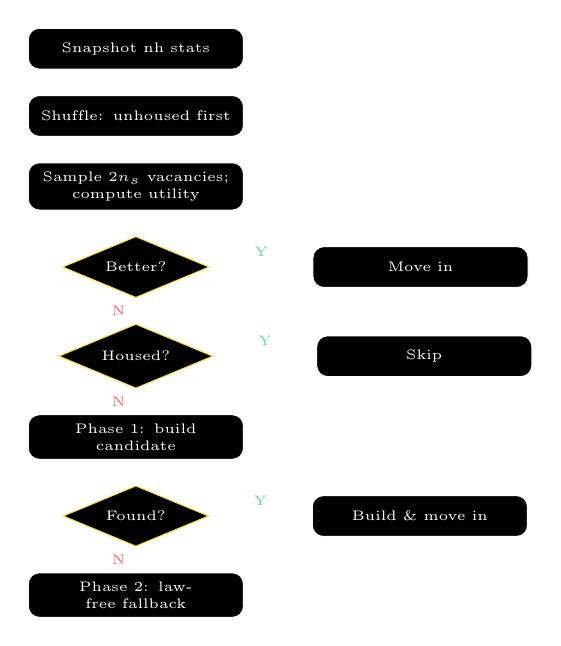
\begin{tikzpicture}[>=Stealth, scale=0.82,
      node distance=0.32cm and 1.0cm,
      box/.style={draw=white, rounded corners, fill=black, text=white,
                  font=\tiny, text width=2.5cm, align=center, minimum height=0.52cm},
      decision/.style={draw=nimbyyellow, diamond, aspect=2.4, fill=black, text=white,
                       font=\tiny, align=center},
      arr/.style={->, thick, white}]
    \node[box] (snap)   {Snapshot nh stats};
    \node[box, below=of snap] (shuffle) {Shuffle: unhoused first};
    \node[box, below=of shuffle] (search) {Sample $2n_s$ vacancies; compute utility};
    \node[decision, below=of search] (better) {Better?};
    \node[box, right=1.3cm of better] (move)  {Move in};
    \node[decision, below=of better] (housed) {Housed?};
    \node[box, right=1.3cm of housed] (skip)  {Skip};
    \node[box, below=of housed] (build)  {Phase 1: build candidate};
    \node[decision, below=of build] (found) {Found?};
    \node[box, right=1.3cm of found] (built) {Build \& move in};
    \node[box, below=of found] (p2) {Phase 2: law-free fallback};
    % arrows
    \draw[arr] (snap) -- (shuffle);
    \draw[arr] (shuffle) -- (search);
    \draw[arr] (search) -- (better);
    \draw[arr] (better) -- node[above,font=\tiny,color=nimbygreen]{Y} (move);
    \draw[arr] (better) -- node[left,font=\tiny,color=nimbyred]{N}  (housed);
    \draw[arr] (housed)  -- node[above,font=\tiny,color=nimbygreen]{Y} (skip);
    \draw[arr] (housed)  -- node[left,font=\tiny,color=nimbyred]{N}  (build);
    \draw[arr] (build)   -- (found);
    \draw[arr] (found)   -- node[above,font=\tiny,color=nimbygreen]{Y} (built);
    \draw[arr] (found)   -- node[left,font=\tiny,color=nimbyred]{N}  (p2);
  \end{tikzpicture}
  \end{center}
\end{frame}

% --- slide: NIMBY mechanism ------------------------------------------
\begin{frame}
  \frametitle{The NIMBY Mechanism}
  \begin{columns}
    \column{0.52\textwidth}
    \textbf{Every $T$ steps:}
    \begin{enumerate}
      \small
      \item Propose a random depth-2 decision tree over neighborhood observables
      \item Deep-copy city: \textcolor{nimbygreen}{with law} vs \textcolor{nimbyred}{without law}
      \item Run $H$ steps of new inflow on each branch (same RNG seed)
      \item Incumbent residents compare utility across branches
      \item Majority vote: if $>50\%$ prefer the law branch $\Rightarrow$ law adopted
    \end{enumerate}
    \column{0.48\textwidth}
    \begin{center}
    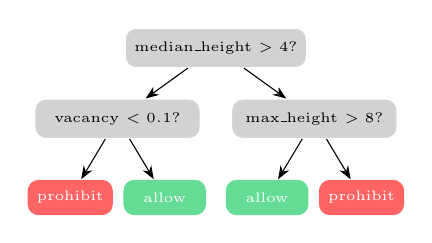
\begin{tikzpicture}[>=Stealth,
        sq/.style={draw=white, fill=gray!35, text=black,
                   rounded corners, minimum width=2.1cm, minimum height=0.5cm,
                   align=center, font=\tiny},
        leaf/.style={rounded corners, text=white,
                     minimum width=1.05cm, minimum height=0.45cm,
                     align=center, font=\tiny}]
      \node[sq] (root) at (0,2.4)     {median\_height $> 4$?};
      \node[sq] (l1)   at (-1.25,1.5) {vacancy $< 0.1$?};
      \node[sq] (r1)   at ( 1.25,1.5) {max\_height $> 8$?};
      \node[leaf, fill=nimbyred]   (ll) at (-1.85,0.5) {prohibit};
      \node[leaf, fill=nimbygreen] (lr) at (-0.65,0.5) {allow};
      \node[leaf, fill=nimbygreen] (rl) at ( 0.65,0.5) {allow};
      \node[leaf, fill=nimbyred]   (rr) at ( 1.85,0.5) {prohibit};
      \draw[->] (root) -- node[left, font=\tiny,color=white]{Y} (l1);
      \draw[->] (root) -- node[right,font=\tiny,color=white]{N} (r1);
      \draw[->] (l1) -- node[left, font=\tiny,color=white]{Y} (ll);
      \draw[->] (l1) -- node[right,font=\tiny,color=white]{N} (lr);
      \draw[->] (r1) -- node[left, font=\tiny,color=white]{Y} (rl);
      \draw[->] (r1) -- node[right,font=\tiny,color=white]{N} (rr);
    \end{tikzpicture}
    \end{center}
    \end{columns}
  \vspace{0.3em}
  \small Laws are \textbf{conditional}: the same law may allow building in one period, block it in another.
\end{frame}

% --- slide: transport and employer -----------------------------------
\begin{frame}
  \frametitle{Transport Network \& Employer}
  \begin{columns}
    \column{0.5\textwidth}
    \textbf{Roads (BFS hop cache):}
    \begin{itemize}
      \small
      \item Neighborhoods connected by a road network
      \item Effective distance $= \min(\text{Euclidean},\; d_{\text{subway}})$
      \item Subway $= $ walk to hub $+$ hops $\times$ road unit $+$ walk from hub
      \item Greedy road planner adds highest-contrast edges
    \end{itemize}
    \column{0.5\textwidth}
    \textbf{Employer (branch simulation):}
    \begin{itemize}
      \small
      \item Single employer tracks all worker IDs
      \item Every $T_e$ steps: sample $k$ candidate buildings
      \item Deep-copy and run $H_e$ steps on each candidate
      \item Relocate to minimise mean effective commute
    \end{itemize}
  \end{columns}
  \vspace{0.5em}
  \begin{center}
  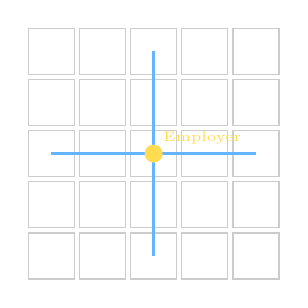
\begin{tikzpicture}[scale=0.65]
    % simple 5x5 nh grid with road overlay
    \foreach \x in {0,...,4} \foreach \y in {0,...,4} {
      \draw[gray!40] (\x,\y) rectangle (\x+0.9,\y+0.9);
    }
    % road segments
    \foreach \x in {0,...,3} {
      \draw[nimbyblue, very thick] (\x+0.45,2.45) -- (\x+1.45,2.45); % horizontal road
    }
    \foreach \y in {0,...,3} {
      \draw[nimbyblue, very thick] (2.45,\y+0.45) -- (2.45,\y+1.45); % vertical road
    }
    % employer
    \fill[nimbyyellow] (2.45,2.45) circle (5pt) node[above right, font=\tiny, color=nimbyyellow]{Employer};
  \end{tikzpicture}
  \end{center}
\end{frame}

% --- slide: emergent behaviors ---------------------------------------
\begin{frame}
  \frametitle{What Emerges}
  \begin{enumerate}
    \item \textcolor{nimbygreen}{\textbf{Sorting}} — agents self-segregate by density preference
    \item \textcolor{nimbyyellow}{\textbf{Height cascades}} — successful tall buildings attract similar agents, law proposals struggle
    \item \textcolor{nimbyred}{\textbf{Law persistence}} — once a restrictive law passes, neighborhood stays low-density
    \item \textcolor{nimbyblue}{\textbf{Employer drift}} — job center migrates toward high-density worker clusters
    \item \textcolor{white}{\textbf{Unhoused fraction}} — regulated cities produce persistent homelessness even with empty land
  \end{enumerate}
\end{frame}

% =====================================================================
%  SECTION 3 — GENERATIVE AI
% =====================================================================

\begin{frame}
  \frametitle{Building with Generative AI}
  \begin{center}
    \textcolor{nimbygray}{$\approx$1,500 lines of Julia $+$ Python $+$ HTML across 10 files}\\[0.5em]
    \textcolor{nimbygray}{Real-time WebSocket visualization, branch-simulated voting, BFS road cache}\\[1em]
    \textcolor{nimbyyellow}{\large Built over $\sim$9 sessions with Claude as collaborator}
  \end{center}
\end{frame}

\begin{frame}
  \frametitle{How AI Was Used}
  \begin{columns}
    \column{0.5\textwidth}
    \textcolor{nimbygreen}{\textbf{Architecture}}
    \begin{itemize}
      \small
      \item Struct design (City, Agent, Law, Employer)
      \item WebSocket protocol between Julia $\leftrightarrow$ Blender $\leftrightarrow$ browser
      \item Frank copula parameterisation
    \end{itemize}
    \vspace{0.5em}
    \textcolor{nimbyblue}{\textbf{Implementation}}
    \begin{itemize}
      \small
      \item Boilerplate (BFS, JSON serialisation)
      \item Debugging async race conditions
      \item Blender mesh geometry API
    \end{itemize}
    \column{0.5\textwidth}
    \textcolor{nimbyyellow}{\textbf{What AI does not replace}}
    \begin{itemize}
      \small
      \item Model design choices (what \emph{should} agents optimize?)
      \item Identifying economically meaningful bugs
      \item Interpreting simulation output
      \item Deciding which parameters to sweep
    \end{itemize}
  \end{columns}
\end{frame}

\begin{frame}
  \frametitle{A Concrete Example: The Employer Bug}
  \begin{enumerate}
    \item Employer initialized at building ID 1 — grid corner $(0,0)$
    \item All 5,000 agents assigned job there
    \item Agents clustered at corner; single tower $>200$ floors
    \item AI spotted the bug when shown the output: \textcolor{nimbyyellow}{``employer should start at the city centroid''}
    \item Fix: compute nearest building to $\left(\frac{n_x \cdot k}{2},\; \frac{n_y \cdot k}{2}\right)$
  \end{enumerate}
  \vspace{0.5em}
  \small The bug was \emph{economically obvious} in the output but invisible in the code.\\
  AI found it by reasoning about \emph{intent}, not just syntax.
\end{frame}

\begin{frame}
  \frametitle{What Worked and What Required Care}
  \begin{columns}
    \column{0.5\textwidth}
    \textcolor{nimbygreen}{\textbf{Worked well}}
    \begin{itemize}
      \small
      \item Iterative refinement: ``make roads thin and black''
      \item Explaining intent, not code
      \item AI as a persistent memory of the codebase
      \item Catching off-by-one and async bugs
    \end{itemize}
    \column{0.5\textwidth}
    \textcolor{nimbyred}{\textbf{Required human judgment}}
    \begin{itemize}
      \small
      \item Verifying economic logic (copula signs, utility direction)
      \item AI over-engineers without constraints
      \item Hallucinated API calls (Blender Python)
      \item Deciding what the model is \emph{for}
    \end{itemize}
  \end{columns}
  \vspace{0.7em}
  \begin{center}
    \textcolor{nimbyyellow}{AI accelerates implementation; it does not replace the researcher.}
  \end{center}
\end{frame}

% =====================================================================
%  SECTION 4 — PARAMETER SWEEPS
% =====================================================================

\begin{frame}
  \frametitle{Research Questions for the Sweep}
  \begin{enumerate}
    \item How does \textcolor{nimbyblue}{preference correlation} ($\theta$) affect law adoption rates?
    \item Does a \textcolor{nimbyyellow}{longer voting horizon} ($H$) produce more or less restrictive cities?
    \item When does the city tip from \textcolor{nimbygreen}{low-density equilibrium} to \textcolor{nimbyred}{high-density equilibrium}?
    \item What is the \textcolor{white}{unhoused fraction} as a function of law frequency?
  \end{enumerate}
\end{frame}

\begin{frame}
  \frametitle{Parameter Sweep Design}
  \begin{center}
  \renewcommand{\arraystretch}{1.3}
  \begin{tabular}{llll}
    \toprule
    \textcolor{nimbygray}{Parameter} & \textcolor{nimbygray}{Meaning} & \textcolor{nimbygray}{Values} & \textcolor{nimbygray}{Axis} \\
    \midrule
    $\theta_\mu$ & copula dependence & 0.5, 2, 5, 10 & A \\
    $H$ & law eval horizon & 5, 10, 20 & B \\
    $T$ & law eval every $N$ steps & 5, 10, 20 & C \\
    $\sigma^{nh}_\mu$ (log) & density sensitivity & $-1, -0.5, 0, 0.5$ & D \\
    \bottomrule
  \end{tabular}
  \end{center}
  \vspace{0.5em}
  \textbf{Focused design}: sweep axes A $\times$ B (4$\times$3 = 12 cells)\\
  $\times$ 3 replications $\times$ 200 steps each = \textbf{36 runs overnight}\\[0.3em]
  Fix $T=10$, $\sigma^{nh}_\mu = -0.5$ (tight preferences); vary $\theta$ and $H$.\\[0.5em]
  \small Outcome variables: \% neighborhoods with active law, mean height, unhoused \%, employer displacement.
\end{frame}

% --- result placeholder: heatmap ------------------------------------
\begin{frame}
  \frametitle{Expected Result: Law Adoption Heatmap}
  \begin{center}
  % Pure TikZ heatmap — no matrix plot* dependency
  % Rows = H (horizon), Cols = theta.  Value = % nh with active law (PLACEHOLDER).
  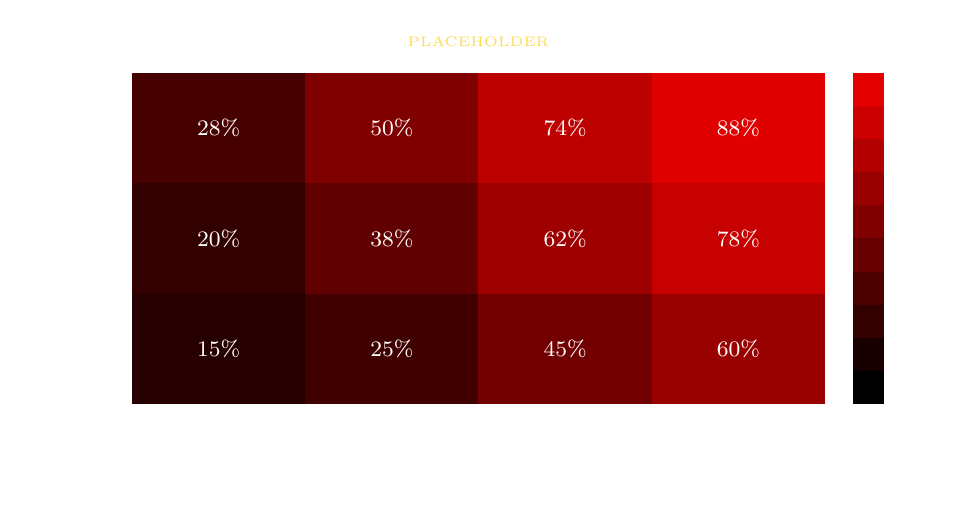
\begin{tikzpicture}[font=\small]
    \def\cw{2.2}  % cell width
    \def\ch{1.4}  % cell height
    % Data: {col/row/value} — col 0-3 = θ ∈ {0.5,2,5,10}, row 0-2 = H ∈ {5,10,20}
    \foreach \col/\row/\val in {
        0/0/15, 1/0/25, 2/0/45, 3/0/60,
        0/1/20, 1/1/38, 2/1/62, 3/1/78,
        0/2/28, 1/2/50, 2/2/74, 3/2/88} {
      \fill[red!\val!black]
        (\col*\cw, \row*\ch) rectangle (\col*\cw+\cw, \row*\ch+\ch);
      \node[white, font=\footnotesize] at (\col*\cw+\cw/2, \row*\ch+\ch/2)
        {\val\%};
    }
    % Column labels (θ)
    \foreach \col/\lbl in {0/$0.5$, 1/$2$, 2/$5$, 3/$10$} {
      \node[white, below, font=\small] at (\col*\cw+\cw/2, 0) {\lbl};
    }
    % Row labels (H)
    \foreach \row/\lbl in {0/$5$, 1/$10$, 2/$20$} {
      \node[white, left, font=\small] at (0, \row*\ch+\ch/2) {\lbl};
    }
    % Axis titles
    \node[white, below=0.55cm, font=\small] at (2*\cw, 0)
      {Copula dependence $\theta_\mu$};
    \node[white, rotate=90, font=\small] at (-1.1, 1.5*\ch)
      {Horizon $H$};
    % Colour scale bar (right side)
    \foreach \i in {0,1,...,9} {
      \fill[red!\i0!black]
        (4*\cw+0.35, \i*3*\ch/10) rectangle (4*\cw+0.75, \i*3*\ch/10+3*\ch/10);
    }
    \node[white, font=\tiny, right] at (4*\cw+0.75, 0)       {0\%};
    \node[white, font=\tiny, right] at (4*\cw+0.75, 3*\ch)    {100\%};
    \node[nimbyyellow, font=\tiny]  at (2*\cw, 3*\ch+0.4)     {PLACEHOLDER};
  \end{tikzpicture}
  \end{center}
  \small Higher $\theta$ and longer horizon $\Rightarrow$ more restrictive laws.
\end{frame}

% --- result placeholder: line plot ----------------------------------
\begin{frame}
  \frametitle{Expected Result: Unhoused Fraction vs.\ Law Frequency}
  \begin{center}
  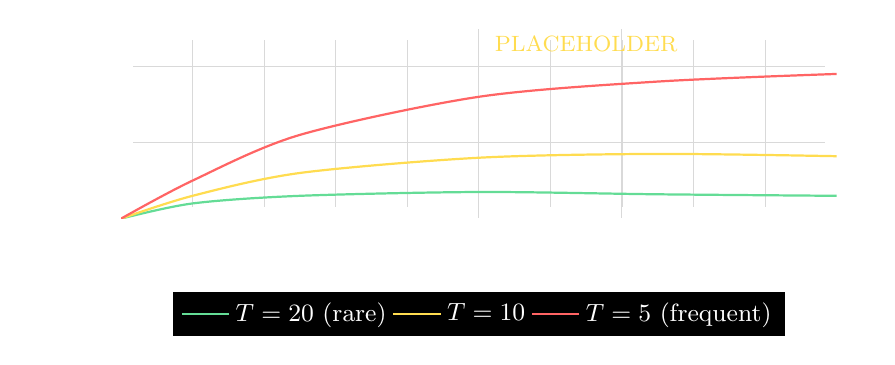
\begin{tikzpicture}
    \begin{axis}[
      width=0.88\textwidth, height=4.0cm,
      xlabel={Simulation step}, ylabel={Unhoused (\%)},
      xmin=0, xmax=200, ymin=0, ymax=25,
      tick style={color=white}, axis line style={color=white},
      xlabel style={color=white}, ylabel style={color=white},
      xticklabel style={color=white}, yticklabel style={color=white},
      grid=major, grid style={color=gray!30},
      legend style={fill=black, draw=white, text=white, font=\small,
                    at={(0.5,-0.38)}, anchor=north, legend columns=-1},
    ]
      \addplot[nimbygreen, thick, smooth] coordinates {
        (0,0)(20,2)(50,3)(100,3.5)(150,3.2)(200,3.0)};
      \addlegendentry{$T=20$ (rare)}
      \addplot[nimbyyellow, thick, smooth] coordinates {
        (0,0)(20,3)(50,6)(100,8)(150,8.5)(200,8.2)};
      \addlegendentry{$T=10$}
      \addplot[nimbyred, thick, smooth] coordinates {
        (0,0)(20,5)(50,11)(100,16)(150,18)(200,19)};
      \addlegendentry{$T=5$ (frequent)}
      \node[color=nimbyyellow, font=\footnotesize] at (axis cs:130,23)
        {PLACEHOLDER};
    \end{axis}
  \end{tikzpicture}
  \end{center}
\end{frame}

% --- result placeholder: scatter ------------------------------------
\begin{frame}
  \frametitle{Expected Result: Employer Displacement vs.\ Law Density}
  \begin{center}
  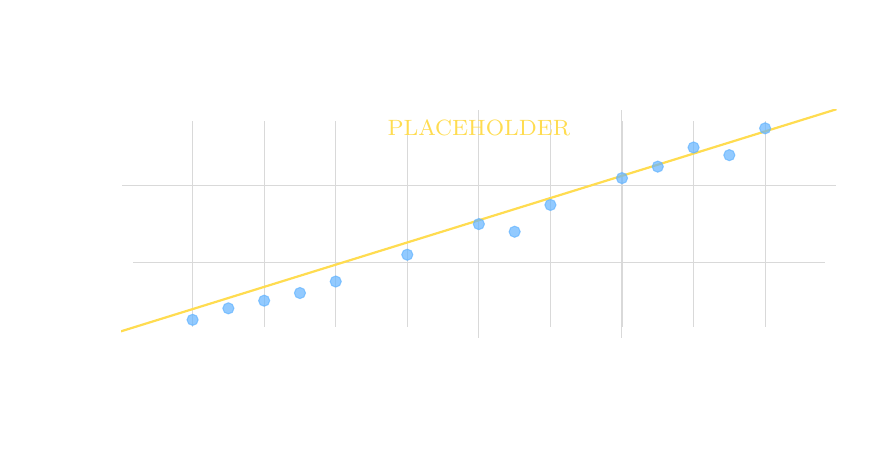
\begin{tikzpicture}
    \begin{axis}[
      width=0.88\textwidth, height=4.5cm,
      xlabel={\% neighborhoods with active law},
      ylabel={Employer displacement (bldgs)},
      xmin=0, xmax=100, ymin=0, ymax=60,
      tick style={color=white}, axis line style={color=white},
      xlabel style={color=white}, ylabel style={color=white},
      xticklabel style={color=white}, yticklabel style={color=white},
      grid=major, grid style={color=gray!30},
    ]
      % PLACEHOLDER scatter
      \addplot[only marks, mark=*, mark size=2pt,
               color=nimbyblue, opacity=0.7] coordinates {
        (10,5)(15,8)(20,10)(25,12)(30,15)(40,22)(50,30)
        (55,28)(60,35)(70,42)(75,45)(80,50)(85,48)(90,55)
      };
      \addplot[nimbyyellow, thick, domain=0:100] {0.58*x + 2};
      \node[color=nimbyyellow, font=\footnotesize] at (axis cs:50,55)
        {PLACEHOLDER};
    \end{axis}
  \end{tikzpicture}
  \end{center}
  \small More laws $\Rightarrow$ employer pushed further from initial location.
\end{frame}

% =====================================================================
%  SECTION 5 — CONNECTIONS AND FUTURE WORK
% =====================================================================

\begin{frame}
  \frametitle{Connection to the Real Market}
  \begin{enumerate}
    \item \textbf{NIMBY} mechanisms protect incumbent interests at the neighborhood scale:\\
      \textcolor{nimbygray}{incumbents vote to restrict new supply, preserving neighborhood character and property values}
    \item This produces \textcolor{nimbyred}{supply restriction} $\Rightarrow$ elevated prices $+$ reduced volume
    \item ABM captures the \textcolor{nimbygreen}{feedback}: laws slow supply $\Rightarrow$ prices rise $\Rightarrow$ incumbents have more to protect $\Rightarrow$ laws tighten
    \item Fairfax County is a natural calibration target: documented high regulatory burden, post-2021 price stickiness
  \end{enumerate}
\end{frame}

\begin{frame}
  \frametitle{Zoning Laws Are Already Trees}
  \begin{columns}
    \column{0.52\textwidth}
    \textcolor{nimbyyellow}{\textbf{An experiment:}} fed the full Fairfax County
    zoning ordinance to ChatGPT and asked:\\[0.4em]
    \textit{``To what extent can these rules be represented as decision trees?''}
    \vspace{0.4em}
    \begin{itemize}
      \small
      \item \textcolor{nimbygreen}{\textbf{Most can}} — permit thresholds, setbacks,
        height limits, and use-by-right tables all branch on observable lot and
        neighborhood attributes
      \item \textcolor{nimbyred}{\textbf{Main exception:}} special-purpose and
        planned-development districts, which require case-by-case negotiation
    \end{itemize}
    \column{0.48\textwidth}
    \textcolor{nimbyblue}{\textbf{Why this matters computationally:}}
    \begin{itemize}
      \small
      \item Zone types map naturally to Julia \textbf{structs}
      \item \textbf{Multiple dispatch} lets different law types share a single
        \texttt{can\_build\_in\_neighborhood} interface — no \texttt{if/else} towers
      \item Opens a path to a \textbf{synthetic Fairfax County}: parameterise
        the model directly from the ordinance, match the observed height and
        vacancy distribution
    \end{itemize}
  \end{columns}
\end{frame}

\begin{frame}
  \frametitle{Future Work}
  \begin{columns}
    \column{0.5\textwidth}
    \textbf{Model extensions}
    \begin{itemize}
      \small
      \item Heterogeneous employers (job clusters, not a single center)
      \item Realtor agent coordinating buyer/seller matching
      \item Demographic aging (cohort-based entry/exit)
    \end{itemize}
    \column{0.5\textwidth}
    \textbf{Calibration}
    \begin{itemize}
      \small
      \item Fairfax County parcel data $\Rightarrow$ building height distribution
      \item HMDA data $\Rightarrow$ agent budget distribution
      \item Zoning board records $\Rightarrow$ law adoption frequency
      \item Moment-matching on median price trajectory
    \end{itemize}
  \end{columns}
\end{frame}

% =====================================================================
%  SECTION 6 — CONCLUSION
% =====================================================================

\begin{frame}
  \frametitle{Summary}
  \begin{enumerate}
    \item \textcolor{nimbyblue}{\textbf{Empirically}}: NIMBY zoning explains post-2022 price stickiness in tight markets
    \item \textcolor{nimbygreen}{\textbf{The ABM}}: heterogeneous agents sort, build, vote on laws, and drive employer location — rich emergent dynamics
    \item \textcolor{nimbyyellow}{\textbf{AI as collaborator}}: accelerates implementation; human judgment still required for model design and interpretation
    \item \textcolor{nimbyred}{\textbf{Parameter sweeps}}: higher preference correlation and longer voting horizons both amplify law adoption and unhoused fractions
    \item \textcolor{white}{\textbf{Next step}}: deepen the bridge between model mechanics and real urban policy
  \end{enumerate}
\end{frame}

\begin{frame}
  \frametitle{Thank You}
  \begin{center}
    \textcolor{nimbygray}{\large John S. Schuler}\\[0.4em]
    \textcolor{white}{jschule4@gmu.edu}\\[1em]
    \textcolor{nimbygray}{Department of Computational and Data Sciences\\
    George Mason University}\\[1.5em]
    \textcolor{nimbyyellow}{Code: \texttt{github.com/jsschuler/urban1}}\\[1em]
    \small Questions welcome on: ABM design $\cdot$ AI-assisted research $\cdot$ parameter sweep results
  \end{center}
\end{frame}

\end{document}
